\chapter{Writing Cookbooks}

A cookbook is the fundamental unit of configuration and policy distribution. Each cookbook defines a scenario, such as everything needed to install and configure MySQL, and then it contains all of the components that are required to support that scenario.

As you read from previous chapter vendor cookbooks can help you to install and configure any possible software, but in most cases it is not enough. This is because you have you application, which need install, configure special cases only for this application. What is why you must to know how to write own Chef cookbooks.

Chef cookbooks is written on \href{https://www.ruby-lang.org}{Ruby} language. It is dynamic and open source programming language, which very well fit to use as \href{http://en.wikipedia.org/wiki/Domain-specific\_language}{DSL} for Chef recipes.

\section{Cookbook file organization}

For beginning we will generate cokbook by knife or berks. You can install both by bundler (we already did this in our kitchens). So, let's create <<my\_cool\_app>> cookbook:

\begin{lstlisting}[language=Bash,label=lst:cookbook-organization1]
$ cd site-cookbooks
$ knife cookbook create my_cool_app -o .
# or another way by berks
$ berks cookbook my_cool_app
\end{lstlisting}

After this you should see inside <<site-cookbooks>> new folder <<my\_cool\_app>>. This is our cookbook, which have such file structure inside:

\begin{lstlisting}[language=Bash,label=lst:cookbook-organization2]
$ ls -l my_cool_app
total 72
drwxr-xr-x  .
drwxr-xr-x  ..
drwxr-xr-x  .git
-rw-r--r--  .gitignore
-rw-r--r--  Berksfile
-rw-r--r--  Gemfile
-rw-r--r--@ LICENSE
-rw-r--r--  README.md
-rw-r--r--  Thorfile
-rw-r--r--  Vagrantfile
drwxr-xr-x  attributes
-rw-r--r--  chefignore
drwxr-xr-x  definitions
drwxr-xr-x  files
drwxr-xr-x  libraries
-rw-r--r--  metadata.rb
drwxr-xr-x  providers
drwxr-xr-x  recipes
drwxr-xr-x  resources
drwxr-xr-x  templates
\end{lstlisting}

Let's consider this structure:

\begin{itemize}
  \item \textbf{.git} - git repository skeleton (no need to do <<git init>>)
  \item \textbf{.gitignore} - specifies intentionally untracked files to ignore by Git
  \item \textbf{Berksfile} - file with cookbook dependencies for berkshelf (used for testing)
  \item \textbf{Gemfile} - file with gems for bundler (used for testing)
  \item \textbf{LICENSE} - file contain license information about cookbook
  \item \textbf{README.md} - file contains information about cookbook. <<.md>> mean \href{http://daringfireball.net/projects/markdown/syntax}{markdown} syntax
  \item \textbf{Thorfile} - file include tasks for thor gem (toolkit for building command-line interfaces, used for testing)
  \item \textbf{Vagrantfile} - file describe the type of machine required for a cookbook for vagrant
  \item \textbf{attributes} - this folder contain ruby files with default cookbook attributes, which you can redefine in environment, role or node attributes
  \item \textbf{chefignore} - specifies intentionally untracked files to ignore by Chef, Knife
  \item \textbf{definitions} - this folder contain ruby files which is used to declare resources so they can be added to the resource collection
  \item \textbf{files} - this folder contain files, which just need transfer to node (used by command <<cookbook\_file>>)
  \item \textbf{libraries} - this folder contain ruby files with Ruby code to be included in a cookbook, either as a way to extend the classes used by the chef-client or to implement a new class directly
  \item \textbf{metadata.rb} - a file, which contain all information (metadata) about the cookbook: name, dependencies, etc. (it is like gemset for ruby gems, package.json for npm, etc)
  \item \textbf{providers} - this folder contain providers for chef resources
  \item \textbf{recipes} - this folder contain recipes of this cookbook
  \item \textbf{resources} - this folder contain resources for chef (like build-in cron, deploy, etc)
  \item \textbf{templates} - this folder contain files written in a markup language that allows the contents of a file to be dynamically generated based on variables or complex logic. Used an Embedded Ruby (ERB) templates.
\end{itemize}

\section{Metadata}

Metadata is file, which contain all main information about cookbook. Let's consider our generated example:

\begin{lstlisting}[label=lst:cookbook-metadata1,title=my-server-cloud/site-cookbooks/my\_cool\_app/metadata.rb]
name             'my_cool_app'
maintainer       'YOUR_NAME'
maintainer_email 'YOUR_EMAIL'
license          'All rights reserved'
description      'Installs/Configures my_cool_app'
long_description IO.read(File.join(File.dirname(__FILE__), 'README.md'))
version          '0.1.0'
\end{lstlisting}

This file written on Ruby and can have such settings:

\begin{itemize}
  \item \textbf{name} - the name of the cookbook
  \item \textbf{maintainer} - the name of the person responsible for maintaining a cookbook, either an individual or an organization
  \item \textbf{maintainer\_email} - the email address for the person responsible for maintaining a cookbook. Only one email can be listed here
  \item \textbf{license} - the type of license under which a cookbook is distributed: <<Apache v2.0>>, <<GPL v2>>, <<GPL v3>>, <<MIT>>, or license <<Proprietary - All Rights Reserved>> (default)
  \item \textbf{description} - a short description of a cookbook and its functionality
  \item \textbf{long\_description} - a longer description that ideally contains full instructions on the proper use of a cookbook, including definitions, libraries, dependencies, and so on. In example the contents pulled from <<README.md>> file
  \item \textbf{version} - the current version of a cookbook. Version numbers always follow a simple three-number version sequence
  \item \textbf{attribute} - the list of attributes that are required to configure a cookbook
  \item \textbf{depends} - indicates that a cookbook has a dependency on another cookbook
  \item \textbf{recommends} - adds a dependency on another cookbook that is recommended, but not required
  \item \textbf{suggests} - adds a dependency on another cookbook that is suggested, but not required
  \item \textbf{conflicts} - indicates that a cookbook conflicts with another cookbook or cookbook version
  \item \textbf{grouping} - adds a title and description to a group of attributes within a namespace
  \item \textbf{provides} - adds a recipe, definition, or resource that is provided by this cookbook, should the auto-populated list be insufficient
  \item \textbf{recipe} - a description for a recipe, mostly for cosmetic value within the server user interface
  \item \textbf{replaces} - indicates that this cookbook should replace another (and can be used in-place of that cookbook)
  \item \textbf{supports} - indicates that a cookbook has a supported platform
\end{itemize}

For our cookbook we need little modify it:

\begin{lstlisting}[label=lst:cookbook-metadata2,title=my-server-cloud/site-cookbooks/my\_cool\_app/metadata.rb]
name             'my_cool_app'
maintainer       'Alexey Vasiliev'
maintainer_email 'leopard_ne@inbox.ru'
license          'MIT'
description      'Installs/Configures my_cool_app'
long_description IO.read(File.join(File.dirname(__FILE__), 'README.md'))
version          '0.1.0'
\end{lstlisting}

As of writing this cookbook, we will be adding information to this file on it.

\section{Recipes}

Any cookbook contains recipes. The default recipe inside cookbook have name <<default>>. Let's add our default recipe, which will install \href{http://git-scm.com/}{git}:

\begin{lstlisting}[label=lst:cookbook-recipes1,title=my-server-cloud/site-cookbooks/my\_cool\_app/recipes/default.rb]
#
# Cookbook Name:: my_cool_app
# Recipe:: default
#
# Copyright (C) 2014 Alexey Vasiliev
#
# MIT
#

package 'git'
\end{lstlisting}

As you can see, at the beginning of recipe we have comments about this recipe. Next we add resource <<package>> with argument <<git>>. The <<package>> resource is used to manage packages on the system. For example, on Debian or Ubuntu resource <<package>> will use <<apt-get>> command to install git on system.

Now you should add <<my\_cool\_app>> into run-list to use this cookbook:

\begin{lstlisting}[label=lst:cookbook-recipes2,title=my-server-cloud/nodes/second.example.com.json]
{
  "name": "second.example.com",
  "json_class": "Chef::Node",
  "chef_type": "node",
  "chef_environment": "development",
  "normal": {
    "fqdn": "10.33.33.35"
  },
  "default": {},
  "override": {},
  "run_list": [
    "role[chef-client]",
    "role[nginx]",
    "recipe[my_cool_app]"
  ]
}
\end{lstlisting}

If you using Chef Server, don't forget upload this cookbook and update node on Chef Server by knife.

\begin{lstlisting}[language=Bash,label=lst:cookbook-recipes3]
$ knife cookbook upload my_cool_app
Uploading my_cool_app    [0.1.0]
Uploaded 1 cookbook.
$ knife node from file nodes/second.example.com.json
Updated Node second.example.com!
// on real environment you will execute "knife ssh 'name:second.example.com' 'sudo chef-client' -i ../keys/production.pem -x ubuntu"
$ vagrant provision chef_second_client
INFO: Chef Run complete in 26.935610739 seconds
INFO: Running report handler
\end{lstlisting}

Let's install also \href{http://en.wikipedia.org/wiki/Network\_Time\_Protocol}{ntp} package in the same recipe. Because we have in recipe Ruby syntax, we can little \href{http://ru.wikipedia.org/wiki/Dont\_repeat\_yourself}{DRY} our code:

\begin{lstlisting}[label=lst:cookbook-recipes4,title=my-server-cloud/site-cookbooks/my\_cool\_app/recipes/default.rb]
%w(git ntp).each do |pack|
  package pack
end
\end{lstlisting}

Again upload cookbook and run chef-client:

\begin{lstlisting}[language=Bash,label=lst:cookbook-recipes5]
$ knife cookbook upload my_cool_app
Uploading my_cool_app    [0.1.0]
Uploaded 1 cookbook.
// on real environment you will execute "knife ssh 'name:second.example.com' 'sudo chef-client' -i ../keys/production.pem -x ubuntu"
$ vagrant provision chef_second_client
INFO: Chef Run complete in 26.935610739 seconds
INFO: Running report handler
$ vagrant ssh chef_second_client
...
vagrant@precise64:~$ ps ax | grep ntp
 1115 ?        Ss     0:00 /usr/sbin/ntpd -p /var/run/ntpd.pid -g -u 103:108
13839 pts/2    S+     0:00 grep --color=auto ntp
vagrant@precise64:~$ git --version
git version 1.7.9.5
\end{lstlisting}

As you can see our simple cookbook is working.


\subsection{Assign Dependencies}

If a cookbook has a dependency on a recipe that is located in another cookbook, that dependency must be declared in the metadata.rb file for that cookbook using the depends keyword.

For example, if the following recipe is included in a cookbook named <<my\_app>>:

\begin{lstlisting}[language=Bash,label=lst:cookbook-recipes6]
include_recipe "apache2::mod_ssl"
\end{lstlisting}

Then the metadata.rb file for that cookbook would have:

\begin{lstlisting}[language=Bash,label=lst:cookbook-recipes7]
depends "apache2"
\end{lstlisting}

\subsection{Create Exceptions}

A recipe can write events to a log file and can cause exceptions using \inline{Chef::Log}. The levels include debug, info, warn, error, and fatal. For example, to just capture information:

\begin{lstlisting}[language=Bash,label=lst:cookbook-recipes7]
Chef::Log.info('some useful information')
\end{lstlisting}

Or to trigger a fatal exception:

\begin{lstlisting}[language=Bash,label=lst:cookbook-recipes8]
Chef::Log.fatal!('something bad')
\end{lstlisting}

\subsection{Include Recipes}

A recipe can include one (or more) recipes located in external cookbooks by using the \inline{include_recipe} method. When a recipe is included, the resources found in that recipe will be inserted (in the same exact order) at the point where the \inline{include_recipe} keyword is located. The syntax for including a recipe is like this:

\begin{lstlisting}[language=Bash,label=lst:cookbook-recipes9]
include_recipe "recipe"
\end{lstlisting}

For example:

\begin{lstlisting}[language=Bash,label=lst:cookbook-recipes10]
include_recipe "apache2::mod_ssl"
\end{lstlisting}

If the \inline{include_recipe} method is used more than once to include a recipe, only the first inclusion is processed and any subsequent inclusions are ignored.

\subsection{Reload Attributes}

Attributes sometimes depend on actions taken from within recipes, so it may be necessary to reload a given attribute from within a recipe. For example:

\begin{lstlisting}[language=Bash,label=lst:cookbook-recipes11]
ruby_block 'some_code' do
  block do
    node.from_file(run_context.resolve_attribute("COOKBOOK_NAME", "ATTR_FILE"))
  end
  action :nothing
end
\end{lstlisting}

\subsection{Accessor Methods}

Attribute accessor methods are automatically created and the method invocation can be used interchangeably with the keys. For example:

\begin{lstlisting}[language=Bash,label=lst:cookbook-recipes12]
default.apache.dir          = "/etc/apache2"
default.apache.listen_ports = [ "80","443" ]
ion :nothing
end
\end{lstlisting}

This is a matter of style and preference for how attributes are reloaded from recipes, and may be seen when retrieving the value of an attribute.
\section{Resources and Providers}
\label{sec:cookbook-resources}

As you read from previous chapter, Chef inside have resources (in example we used \inline!package! resource). A resource defines the actions that can be taken, such as when a package should be installed, whether a service should be enabled or restarted, which groups, users, or groups of users should be created, where to put a collection of files, what the name of a new directory should be, and so on. During a chef-client run, each resource is identified and then associated with a provider. The provider then does the work to complete the action defined by the resource. Each resource is processed in the same order as they appear in a recipe. The chef-client ensures that the same actions are taken the same way everywhere and that actions produce the same result every time. A resource is implemented within a recipe using Ruby.

Let's look at the most necessary resources.

\subsection{Bash}

The bash resource is used to execute scripts using the Bash interpreter and includes all of the actions and attributes that are available to the execute resource. Example:

\begin{lstlisting}[label=lst:cookbook-resources-bash]
bash "install_something" do
  user "root"
  cwd "/tmp"
  code <<-EOH
  wget http://www.example.com/tarball.tar.gz
  tar -zxf tarball.tar.gz
  cd tarball
  ./configure
  make
  make install
  EOH
end
\end{lstlisting}

\subsection{Cron}

The cron resource is used to manage cron entries for time-based job scheduling. Attributes for a schedule will default to * if not provided. The cron resource requires access to a crontab program, typically cron. Example:

\begin{lstlisting}[label=lst:cookbook-resources-cron1]
cron "name_of_cron_entry" do
  hour "8"
  weekday "6"
  mailto "admin@opscode.com"
  action :create
end
\end{lstlisting}

\begin{lstlisting}[label=lst:cookbook-resources-cron2]
cron "noop" do
  hour "5"
  minute "0"
  command "/bin/true"
end
\end{lstlisting}

\subsection{Directory}

The directory resource is used to manage a directory, which is a hierarchy of folders that comprises all of the information stored on a computer. The root directory is the top-level, under which the rest of the directory is organized. The directory resource uses the name attribute to specify the path to a location in a directory. Typically, permission to access that location in the directory is required. Example:

\begin{lstlisting}[label=lst:cookbook-resources-directory1]
directory "/tmp/something" do
  owner "root"
  group "root"
  mode 00755
  action :create
end
\end{lstlisting}

\begin{lstlisting}[label=lst:cookbook-resources-directory2]
%w{dir1 dir2 dir3}.each do |dir|
  directory "/tmp/mydirs/#{dir}" do
    mode 00775
    owner "root"
    group "root"
    action :create
    recursive true
  end
end
\end{lstlisting}

\subsection{Git}

The git resource is used to manage source control resources that exist in a git repository. git version 1.6.5 (or higher) is required to use all of the functionality in the git resource. Example:

\begin{lstlisting}[label=lst:cookbook-resources-git1]
git "/opt/mysources/couch" do
  repository "git://git.apache.org/couchdb.git"
  reference "master"
  action :sync
end
\end{lstlisting}

\begin{lstlisting}[label=lst:cookbook-resources-git2]
git "#{Chef::Config[:file_cache_path]}/ruby-build" do
 repository "git://github.com/sstephenson/ruby-build.git"
 reference "master"
 action :sync
end

bash "install_ruby_build" do
 cwd "#{Chef::Config[:file_cache_path]}/ruby-build"
 user "rbenv"
 group "rbenv"
 code <<-EOH
   ./install.sh
   EOH
 environment 'PREFIX' => "/usr/local"
end
\end{lstlisting}

\subsection{Link}

The link resource is used to create symbolic or hard links. Example:

\begin{lstlisting}[label=lst:cookbook-resources-cookbook-link1]
link "/tmp/passwd" do
  to "/etc/passwd"
end
\end{lstlisting}

\begin{lstlisting}[label=lst:cookbook-resources-cookbook-link2]
link "/tmp/passwd" do
  to "/etc/passwd"
  link_type :hard
end
\end{lstlisting}

\subsection{Cookbook\_file}

The cookbook\_file resource is used to transfer files from a sub-directory of the files/ directory in a cookbook to a specified path that is located on the host running the chef-client or chef-solo. The file in a cookbook is selected according to file specificity, which allows different source files to be used based on the hostname, host platform (operating system, distro, or as appropriate), or platform version. Files that are located under COOKBOOK\_NAME/files/default can be used on any platform. Example:

\begin{lstlisting}[label=lst:cookbook-resources-cookbook-file1]
cookbook_file "/tmp/testfile" do
  source "testfile"
  mode 00644
end
\end{lstlisting}

\begin{lstlisting}[label=lst:cookbook-resources-cookbook-file2]
cookbook_file "/etc/yum.repos.d/custom.repo" do
  source "custom"
  mode 00644
  notifies :run, "execute[create-yum-cache]", :immediately
  notifies :create, "ruby_block[reload-internal-yum-cache]", :immediately
end
\end{lstlisting}

\subsection{Template}

The template resource is used to manage file contents with an embedded Ruby (erb) template. This resource includes actions and attributes from the file resource. Template files managed by the template resource follow the same file specificity rules as the remote\_file and file resources. Example:

\begin{lstlisting}[label=lst:cookbook-resources-cookbook-template1]
template "/tmp/config.conf" do
  source "config.conf.erb"
end
\end{lstlisting}

\begin{lstlisting}[label=lst:cookbook-resources-cookbook-template2]
template "/tmp/somefile" do
  mode 00644
  source "somefile.erb"
  not_if {File.exists?("/etc/passwd")}
end
\end{lstlisting}

\subsection{Script}

The script resource is used to execute scripts using the specified interpreter (Bash, Csh, Perl, Python, or Ruby) and includes all of the actions and attributes that are available to the execute resource. Example:

\begin{lstlisting}[label=lst:cookbook-resources-cookbook-script1]
script "install_something" do
  interpreter "bash"
  user "root"
  cwd "/tmp"
  code <<-EOH
  wget http://www.example.com/tarball.tar.gz
  tar -zxf tarball.tar.gz
  cd tarball
  ./configure
  make
  make install
  EOH
end
\end{lstlisting}

\subsection{User}

The user resource is used to add users, update existing users, remove users, and to lock/unlock user passwords. Example:

\begin{lstlisting}[label=lst:cookbook-resources-cookbook-user1]
user "random" do
  supports :manage_home => true
  comment "Random User"
  uid 1234
  gid "users"
  home "/home/random"
  shell "/bin/bash"
  password "$1$JJsvHslV$szsCjVEroftprNn4JHtDi."
end
\end{lstlisting}

There are a number of encryption options and tools that can be used to create a password shadow hash. In general, using a strong encryption method like SHA-512 and the passwd command in the OpenSSL toolkit is a good approach, however the encryption options and tools that are available may be different from one distribution to another. The following examples show how the command line can be used to create a password shadow hash. When using the \inline!passwd! command in the OpenSSL tool:

\begin{lstlisting}[language=Bash,label=lst:cookbook-resources-cookbook-user2]
$ openssl passwd -1 "theplaintextpassword"
\end{lstlisting}

Another example:

\begin{lstlisting}[label=lst:cookbook-resources-cookbook-user3]
user "systemguy" do
  comment "system guy"
  system true
  shell "/bin/false"
end
\end{lstlisting}

\subsection{Deploy}

The deploy resource is used to manage and control deployments. This is a popular resource, but is also complex, having the most attributes, multiple providers, the added complexity of callbacks, plus four attributes that support layout modifications from within a recipe.

The deploy resource is modeled after \href{http://capistranorb.com/}{Capistrano}, a utility and framework for executing commands in parallel on multiple remote machines via SSH. The deploy resource is designed to behave in a way that is similar to the \inline!deploy! and \inline!deploy:migration! tasks in Capistrano.
\section{Attributes}
\label{sec:cookbook-attributes}

An attribute can be defined in a cookbook (or a recipe) and then used to override the default settings on a node. When a cookbook is loaded during a chef-client run, these attributes are compared to the attributes that are already present on the node. When the cookbook attributes take precedence over the default attributes, the chef-client will apply those new settings and values during the chef-client run on the node.

An attribute file is located in the \inline{attributes/} sub-directory for a cookbook. When a cookbook is run against a node, the attributes contained in all attribute files are evaluated in the context of the node object. Node methods (when present) are used to set attribute values on a node. For example, the <<apache2>> cookbook contains an attribute file called \inline{default.rb}, which contains the following attributes:

\begin{lstlisting}[label=lst:cookbook-attributes1]
default["apache"]["dir"]          = "/etc/apache2"
default["apache"]["listen_ports"] = [ "80","443" ]
\end{lstlisting}

The use of the node object (node) is implicit in the previous example; the following example defines the node object itself as part of the attribute:

\begin{lstlisting}[label=lst:cookbook-attributes2]
node.default["apache"]["dir"]          = "/etc/apache2"
node.default["apache"]["listen_ports"] = [ "80","443" ]
\end{lstlisting}

In our cookbook <<my\_cool\_app>> we want create directory for web app, add to this directory html file, generate config for nginx and enable this configuration. Let's add all this by using Chef attributes and resources.

\begin{lstlisting}[label=lst:cookbook-attributes3,title=my-server-cloud/site-cookbooks/my\_cool\_app/attributes/default.rb]
default['my_cool_app']['web_dir']       = '/var/www/my_cool_app'
default['my_cool_app']['user']          = 'vagrant'
default['my_cool_app']['name']          = 'my_cool_app'
\end{lstlisting}

\begin{lstlisting}[label=lst:cookbook-attributes4,title=my-server-cloud/site-cookbooks/my\_cool\_app/recipes/default.rb]
# install needed package
%w(git ntp).each do |pack|
  package pack
end

# create directory for web app
directory node['my_cool_app']['web_dir'] do
  owner node['my_cool_app']['user']
  mode "0755"
  recursive true
end

# upload index.html file to web app directory as index.html
cookbook_file "#{node['my_cool_app']['web_dir']}/index.html" do
  owner node['my_cool_app']['user']
  source "index.html"
  mode 0755
end

# create nginx config from temlate nginx.conf.erb
nginx_config = "#{node['nginx']['dir']}" +
  "/sites-available/#{node['my_cool_app']['name']}.conf"
template nginx_config do
  source "nginx.conf.erb"
  mode "0644"
end

# activate nginx.conf in nginx
nginx_site "#{node['my_cool_app']['name']}.conf"
\end{lstlisting}

\begin{lstlisting}[language=HTML,label=lst:cookbook-attributes5,title=my-server-cloud/site-cookbooks/my\_cool\_app/templates/default/nginx.conf.erb]
server {
    listen 80 default;
    charset utf-8;
    root <%= node['my_cool_app']['web_dir'] %>;
}
\end{lstlisting}

\begin{lstlisting}[language=HTML,label=lst:cookbook-attributes6,title=my-server-cloud/site-cookbooks/my\_cool\_app/files/default/index.html]
<!DOCTYPE html>
<html lang="en">
<head>
  <meta charset="utf-8" />
  <meta http-equiv="X-UA-Compatible" content="IE=edge" />
  <title>My cool app</title>
  <meta name="viewport" content="width=device-width, initial-scale=1.0, user-scalable=0, maximum-scale=1.0" />
</head>
<body>
  <h1>This is my cool web app</h1>
</body>
</html>
\end{lstlisting}

\begin{lstlisting}[label=lst:cookbook-attributes7,title=my-server-cloud/site-cookbooks/my\_cool\_app/metadata.rb]
name             'my_cool_app'
maintainer       'Alexey Vasiliev'
maintainer_email 'leopard_ne@inbox.ru'
license          'MIT'
description      'Installs/Configures my_cool_app'
long_description IO.read(File.join(File.dirname(__FILE__), 'README.md'))
version          '0.1.0'

recipe 'my_cool_app',   'Configure my cool app'

depends 'nginx',           '~> 2.2.0'
\end{lstlisting}

As you can see, we add for default attributes for recipe. Better to use for cookbook attribute name as root for all attributes - in this case you will not have problem, if several cookbooks will use similar keys for settings. As you can see all attributes of this cookbook located inside <<my\_cool\_app>> attribute. In recipe we add needed commands to create and activate our index.html. Also we add to metadata information about recipe and dependence to nginx cookbook (because we used inside our recipe <<nginx\_site>> resource). After upload cookbook at Chef server and run chef-client at the second node, we can see results at \href{http://10.33.33.35}{http://10.33.33.35} (Pic~\ref{fig:my_cool_app_index}):

\begin{lstlisting}[language=Bash,label=lst:cookbook-attributes8]
$ knife cookbook upload my_cool_app
Uploading my_cool_app    [0.1.0]
Uploaded 1 cookbook.
// on real environment you will execute "knife ssh 'name:second.example.com' 'sudo chef-client' -i ../keys/production.pem -x ubuntu"
$ vagrant provision chef_second_client
...
INFO: directory[/var/www/my_cool_app] created directory /var/www/my_cool_app
INFO: directory[/var/www/my_cool_app] owner changed to 1000
INFO: directory[/var/www/my_cool_app] mode changed to 755
INFO: cookbook_file[/var/www/my_cool_app/index.html] created file /var/www/my_cool_app/index.html
INFO: cookbook_file[/var/www/my_cool_app/index.html] updated file contents /var/www/my_cool_app/index.html
INFO: cookbook_file[/var/www/my_cool_app/index.html] owner changed to 1000
INFO: cookbook_file[/var/www/my_cool_app/index.html] mode changed to 755
INFO: template[/etc/nginx/sites-available/my_cool_app.conf] created file /etc/nginx/sites-available/my_cool_app.conf
INFO: template[/etc/nginx/sites-available/my_cool_app.conf] updated file contents /etc/nginx/sites-available/my_cool_app.conf
INFO: template[/etc/nginx/sites-available/my_cool_app.conf] mode changed to 644
INFO: execute[nxensite my_cool_app.conf] ran successfully
INFO: execute[nxensite my_cool_app.conf] sending reload action to service[nginx] (delayed)
INFO: service[nginx] reloaded
...
\end{lstlisting}

\begin{figure}[ht!]
  \center{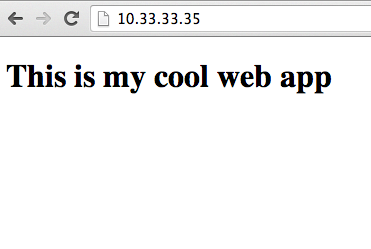
\includegraphics[width=0.6\textwidth]{my_cool_app_index}}
  \caption{Our cool app}
  \label{fig:my_cool_app_index}
\end{figure}
\section{Templates}

As you can see in previous chapter we used resource \inline{template} for generate nginx config in default recipe. A cookbook template is a file written in a markup language that allows the contents of a file to be dynamically generated based on variables or complex logic. Templates can contain Ruby expressions and statements. Templates are a great way to manage configuration files across an organization. A template requires a template resource being added to a recipe and then a corresponding Embedded Ruby (ERB) template being added to a cookbook.

To use a template, two things must happen:

\begin{itemize}
  \item A template resource must be added to a recipe
  \item An Embedded Ruby (ERB) template must be added to a cookbook
\end{itemize}

For example, the following template file and template resource settings can be used to manage a configuration file named \inline{/etc/sudoers}. Within a cookbook that uses sudo, the following resource could be added to \inline{recipes/default.rb}:

\begin{lstlisting}[label=lst:cookbook-templates1]
template "/etc/sudoers" do
  source "sudoers.erb"
  mode 0440
  owner "root"
  group "root"
  variables({
     :sudoers_groups => node[:authorization][:sudo][:groups],
     :sudoers_users => node[:authorization][:sudo][:users]
  })
end
\end{lstlisting}

And then create a template called \inline{sudoers.erb} and save it to \inline{templates/default/sudoers.erb}:

\begin{lstlisting}[label=lst:cookbook-templates2]
#
# /etc/sudoers
#
# Generated by Chef for <%= node[:fqdn] %>
#

Defaults        !lecture,tty_tickets,!fqdn

# User privilege specification
root          ALL=(ALL) ALL

<% @sudoers_users.each do |user| -%>
<%= user %>   ALL=(ALL) <%= "NOPASSWD:" if @passwordless %>ALL
<% end -%>

# Members of the sysadmin group may gain root privileges
%sysadmin     ALL=(ALL) <%= "NOPASSWD:" if @passwordless %>ALL

<% @sudoers_groups.each do |group| -%>
# Members of the group '<%= group %>' may gain root privileges
%<%= group %> ALL=(ALL) <%= "NOPASSWD:" if @passwordless %>ALL
<% end -%>
\end{lstlisting}

And then set the default attributes in \inline{attributes/default.rb}:

\begin{lstlisting}[label=lst:cookbook-templates3]
default["authorization"]["sudo"]["groups"] = [ "sysadmin","wheel","admin" ]
default["authorization"]["sudo"]["users"]  = [ "jerry","greg"]
\end{lstlisting}

When a template is rendered, Ruby expressions and statements are evaluated by the chef-client. The variables listed in the resource’s variables parameter and the node object are evaluated. The chef-client then passes these variables to the template, where they will be accessible as instance variables within the template; the node object can be accessed just as if it were part of a recipe, using the same syntax.

For example, a simple template resource like this:

\begin{lstlisting}[label=lst:cookbook-templates4]
node[:fqdn] = "latte"
template "/tmp/foo" do
  source "foo.erb"
  variables({
    :x_men => "are keen"
  })
end
\end{lstlisting}

And a simple Embedded Ruby (ERB) template like this:

\begin{lstlisting}[label=lst:cookbook-templates5]
The node <%= node[:fqdn] %> thinks the x-men <%= @x_men %>
\end{lstlisting}

Would render something like:

\begin{lstlisting}[label=lst:cookbook-templates6]
The node latte thinks the x-men are keen
\end{lstlisting}

Even though this is a very simple example, the full capabilities of Ruby can be used to tackle even the most complex and demanding template requirements.

\subsection{File Specificity}

A cookbook will frequently be designed to work across many platforms and will often be required to distribute a specific file to a specific platform. A cookbook can be designed to support distributing files across platforms, but ensuring that the right file ends up on each system.

The pattern for file specificity is as follows:

\begin{enumerate}
  \item \inline{host-node[:fqdn]}
  \item \inline{node[:platform]-node[:platform_version]}
  \item \inline{node[:platform]-version_components}: The version string is split on decimals and searched from greatest specificity to least; for example, if the location from the last rule was centos-5.7.1, then centos-5.7 and centos-5 would also be searched.
  \item \inline{node[:platform]}
  \item \inline{default}
\end{enumerate}

The naming of folders within cookbook directories must literally match the host notation used for template specificity matching. For example, if a host is named <<foo.example.com>>, then the folder must be named <<host-foo.example.com>>.

A cookbook may have a \inline{/templates} directory structure like this:

\begin{lstlisting}[language=Bash,label=lst:cookbook-templates7]
templates/
  windows-6.2
  windows-6.1
  windows-6.0
  windows
  default
\end{lstlisting}

and a resource that looks something like the following:

\begin{lstlisting}[label=lst:cookbook-templates8]
template "C:\path\to\file\text_file.txt" do
  source "text_file.txt"
  mode 0755
  owner "root"
  group "root"
end
\end{lstlisting}

This resource would be matched in the same order as the /templates directory structure. For a node named <<host-node-desktop>> that is running Windows 7, the second item would be the matching item and the location:

\begin{lstlisting}[language=Bash,label=lst:cookbook-templates8]
/templates
  windows-6.2/text_file.txt
  windows-6.1/text_file.txt
  windows-6.0/text_file.txt
  windows/text_file.txt
  default/text_file.txt
\end{lstlisting}

\subsection{Partial Templates}

A template can be built in a way that allows it to contain references to one (or more) smaller template files. (These smaller template files are also referred to as partials.) A partial can be referenced from a template file in one of the following ways:

\begin{itemize}
  \item By using the Ruby render method in the template file
  \item By using the template resource and the variables parameter
\end{itemize}

Use the render method in a template to reference a partial template file with the following syntax:

\begin{lstlisting}[language=Bash,label=lst:cookbook-templates9]
<%= render "partial_name.txt.erb", :option => {} %>
\end{lstlisting}

where \inline{partial_name.txt.erb} is the name of the partial template file and \inline{:option} is one (or more) of the following options:

\begin{itemize}
  \item \inline{:cookbook} - by default, a partial template file is assumed to be located in the cookbook that contains the top-level template. Use this option to specify the path to a different cookbook
  \item \inline{:local} - indicates that the name of the partial template file should be interpreted as a path to a file in the local file system or looked up in a cookbook using the normal rules for template files. Set to true to interpret as a path to a file in the local file system and to false to use the normal rules for template files
  \item \inline{:source} - by default, a partial template file is identified by its file name. Use this option to specify a different name or a local path to use (instead of the name of the partial template file)
  \item \inline{:variables} - a hash of \inline{variable_name => value} that will be made available to the partial template file. When this option is used, any variables that are defined in the top-level template that are required by the partial template file must have them defined explicitly using this option
\end{itemize}

For example:

\begin{lstlisting}[language=Bash,label=lst:cookbook-templates10]
<%= render "simple.txt.erb", :variables => {:user => @user }, :local => true %>
\end{lstlisting}



